\documentclass[german]{uebung}

\usepackage{uebung-meta}

%%%%%%%%%%%%%%%%%%%%%%%%%%%%%%%%%%%%%%%%%%%%%%%%%%%%%%%%%%%%%%%%%%%%%%%%%%%%
% README
%%%%%%%%%%%%%%%%%%%%%%%%%%%%%%%%%%%%%%%%%%%%%%%%%%%%%%%%%%%%%%%%%%%%%%%%%%%%

% How to use this:
% 1. Add your data to uebung-meta.sty (you only need to do this once)
% 2. Copy this file and name it something useful
% 3. Set the assignment to the right value
% 4. Use the exercise enviroment to separate your solutions for the different exercises from each other.

% DO NOT CHANGE uebung.cls! If you need more packages just add a new \usepackage somewhere in this file before the \begin{document}

% The commands
% \div and \grad are provided by uebung.cls

% The environment "exercise" takes one parameter (the exercise number). 
% This way you can skip exercises if you like. Example:
% 
% \assignment{3}
% \begin{exercise}{8}
% ...
% \end{exercise}
% 
% The solution to exercise 3.8 (3rd assignment, 8th exercise) goes where 
% the dots are.

% If the total page number shows up as ?? in the footer you need to compile a second time.

% Which assignment is this?
\assignment{1}


\begin{document}

\begin{exercise}{2}
Etwas Mathematik:
% the div is command is provided by uebung.cls
$$\div  \vec{F} = \nabla \cdot \vec{F} = \sum_{i=1}^{3} \frac{\partial F_i}{\partial x_i}$$
Für mehrzeilige Mathematik bietet sich \verb|align*| aus \emph{amsmath} an:
\begin{align*}
(3+5)^2 &= 3^2+2\cdot 3 \cdot 5 + 5^2\\
&= 9 + 30 + 25\\
&= 64
\end{align*}
\end{exercise}

\begin{exercise}{3}
Ein eingebundenes Bild:
\begin{figure}[h]
	\centering
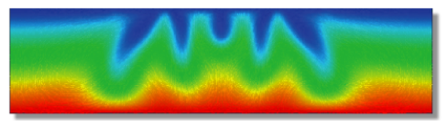
\includegraphics[width=6cm]{image}
	\caption{Beispiel einer eingebundenen Grafik}
\label{fig:grafik}
\end{figure}
\end{exercise}

\begin{exercise}{4}
	Für Grafiken und Plots bietet sich beispielsweise TikZ, eventuell mit pgfplots, an:
	\begin{figure}[h]
		\centering
		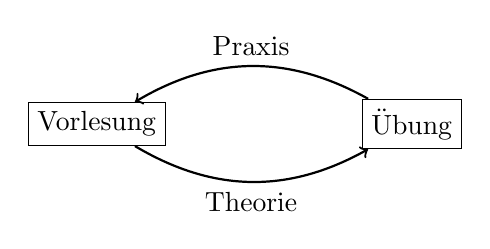
\begin{tikzpicture}
		
		\node[draw,shape=rectangle] (vorl) at (0,0) {Vorlesung};
		\node[draw,shape=rectangle] (uebu) at (4,0) {Übung};
		\draw[->,thick] (vorl)  to[bend right=30] node[below] {Theorie} (uebu) ;
		\draw[->,thick] (uebu)  to[bend right=30] node[above] {Praxis} (vorl) ;
		\end{tikzpicture}
		\caption{Beispiel einer Grafik mit TikZ}
		\label{fig:grafik}
	\end{figure}
	\begin{figure}[h]
		\centering
		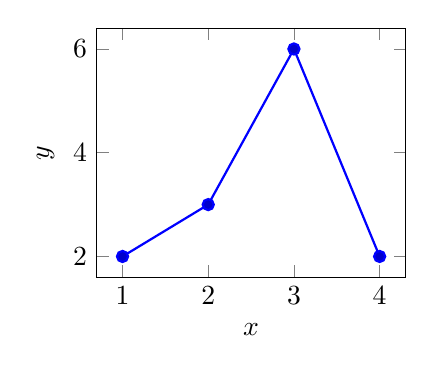
\begin{tikzpicture}
			\begin{axis}[
				xlabel={$x$},
				width=5.5cm,
				ylabel={$y$} ]
				\addplot+[thick,mark=*]
				table [x={x}, y={y}]{ 
					x	 y
					1	2
					2	3
					3	6
					4	2
				};
			\end{axis}
		\end{tikzpicture}
		\caption{Beispiel eines Plots mit TikZ und pgfplots}
		\label{fig:grafik}
	\end{figure}
\end{exercise}


\end{document}
